\documentclass[tikz,border=8pt]{standalone}
\usetikzlibrary{positioning,decorations.pathreplacing}
\begin{document}
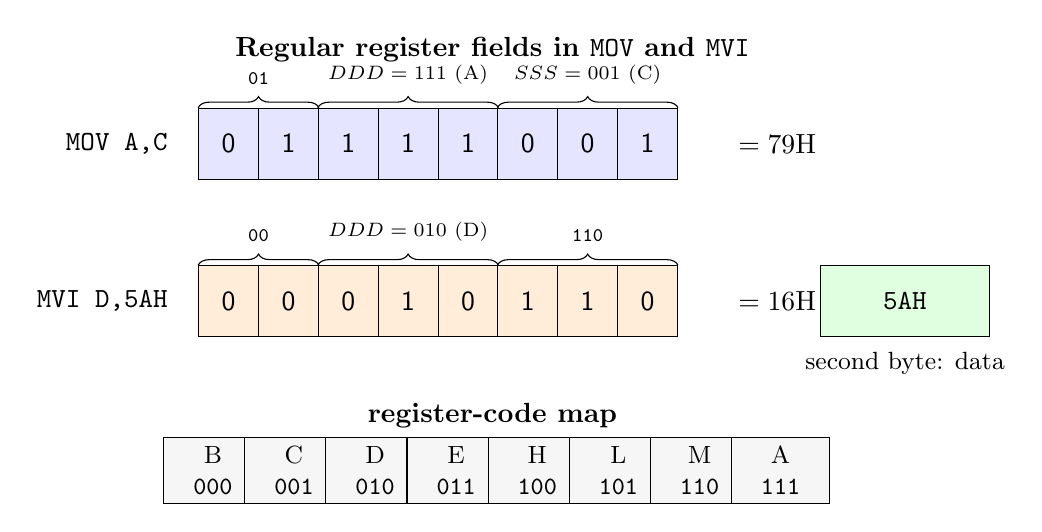
\begin{tikzpicture}[
  font=\sffamily,
  bit/.style={draw,minimum width=0.76cm,minimum height=0.9cm,align=center},
  reg/.style={draw,minimum width=1.25cm,minimum height=0.68cm,align=center,font=\small}
]
\node[font=\bfseries] at (4.0,4.0) {Regular register fields in \texttt{MOV} and \texttt{MVI}};

\node[anchor=east,font=\bfseries] at (0,2.8) {\texttt{MOV A,C}};
\foreach \b [count=\i from 0] in {0,1,1,1,1,0,0,1}{
  \node[bit,fill=blue!10] (m\i) at (0.65+0.76*\i,2.8) {\b};
}
\draw[decorate,decoration={brace,amplitude=4pt}] (m0.north west) -- (m1.north east)
  node[midway,above=5pt,font=\scriptsize] {\texttt{01}};
\draw[decorate,decoration={brace,amplitude=4pt}] (m2.north west) -- (m4.north east)
  node[midway,above=5pt,font=\scriptsize] {$DDD=111$ (A)};
\draw[decorate,decoration={brace,amplitude=4pt}] (m5.north west) -- (m7.north east)
  node[midway,above=5pt,font=\scriptsize] {$SSS=001$ (C)};
\node[anchor=west] at (7.0,2.8) {$=79\mathrm{H}$};

\node[anchor=east,font=\bfseries] at (0,0.8) {\texttt{MVI D,5AH}};
\foreach \b [count=\i from 0] in {0,0,0,1,0,1,1,0}{
  \node[bit,fill=orange!15] (v\i) at (0.65+0.76*\i,0.8) {\b};
}
\draw[decorate,decoration={brace,amplitude=4pt}] (v0.north west) -- (v1.north east)
  node[midway,above=5pt,font=\scriptsize] {\texttt{00}};
\draw[decorate,decoration={brace,amplitude=4pt}] (v2.north west) -- (v4.north east)
  node[midway,above=5pt,font=\scriptsize] {$DDD=010$ (D)};
\draw[decorate,decoration={brace,amplitude=4pt}] (v5.north west) -- (v7.north east)
  node[midway,above=5pt,font=\scriptsize] {\texttt{110}};
\node[anchor=west] at (7.0,0.8) {$=16\mathrm{H}$};
\node[bit,fill=green!12,minimum width=2.15cm,right=1.8cm of v7] (imm) {\texttt{5AH}};
\node[below=2pt of imm,font=\small] {second byte: data};

\node[font=\bfseries] at (4.0,-0.65) {register-code map};
\foreach \name/\code [count=\i from 0] in {B/000,C/001,D/010,E/011,H/100,L/101,M/110,A/111}{
  \node[reg,fill=gray!7] at (0.45+1.03*\i,-1.35) {\name\\\texttt{\code}};
}
\node[below=4mm of v3,font=\small,align=center] {};
\end{tikzpicture}
\end{document}
